\chapter{Implementation of Concurrent Indirect GPU-FPGA Communication}
\label{section:concurrent}

While direct device to device communication is in theory always the fastest possible method, it is more cumbersome to use, requires unofficial modified drivers and is only available for NVIDIA Quadro and Tesla graphics cards.
The indirect method that involves a round-trip via the CPU on the other hand can be simply implemented in standard OpenCL, also with the more popular GeForce cards.
This section describes a naive version and an optimization that can be applied for large transfers

The simplest possible procedure of an indirect transfer can be summarized as follows:
\begin{enumerate}
	\item Read data from the first device into a CPU buffer
	\item Wait until the transfer is done
	\item Send data from the CPU buffer to the second device
\end{enumerate}

In OpenCL this can easily be accomplished in only two lines of code (error checking omitted):
%TODO: code listing
\begin{lstlisting}[label=sequential_indirect,caption=Sequential indirect device to device transfer in OpenCL]
clEnqueueReadBuffer (queue_device1, buffer_device1, CL_TRUE, 
                            0, size, cpu_buffer, 0, NULL, NULL);
clEnqueueWriteBuffer(queue_device2, buffer_device2, CL_TRUE, 
                            0, size, cpu_buffer, 0, NULL, NULL);
\end{lstlisting}

However, this is highly inefficient because at any time one of the two devices is not doing anything.

Both, the GPU as well as the FPGA have one DMA controller.
Both can operate independently of each other.
By splitting up a large transfer into multiple small transfers, one DMA controller can read from a portion of the temporary CPU buffer while the other one is simultaneously writing to the next portion.
This results in an overall faster transfer, as illustrated in figure \ref{fig:concurrent1}.


\begin{figure}[htb]
	  \centerline{
		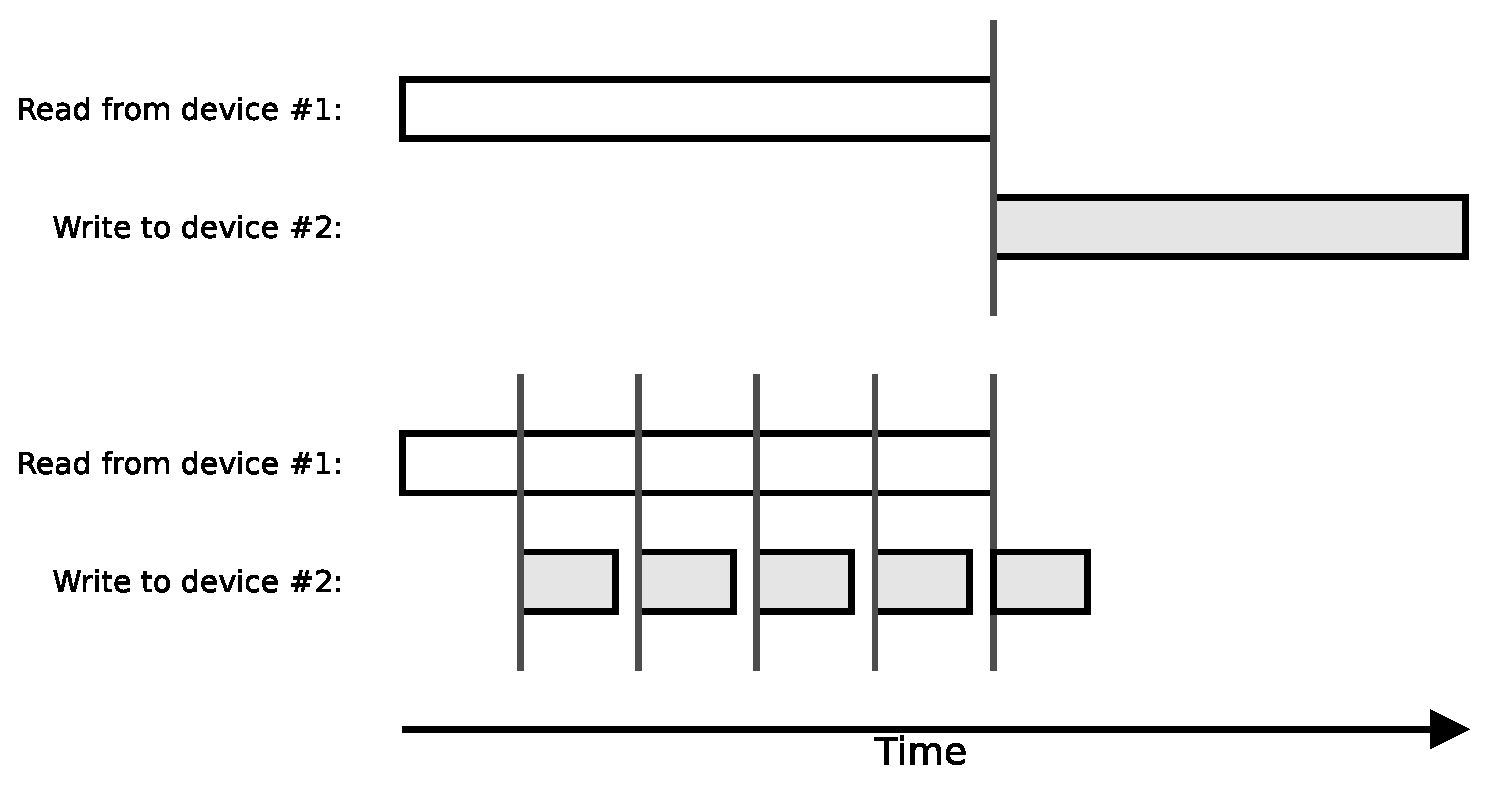
\includegraphics[width=1.0\textwidth]{images/concurrent1.eps}}
	  \caption{Comparison of sequential (top) and concurrent (bottom) indirect transfer strategies. The two large transfers are splitted into 10 smaller transfers, 8 of them can be performed simultaneously. The gray vertical lines represent synchronization barriers.}
	  \label{fig:concurrent1}
\end{figure}


An important parameter is the size and number of the smaller transfers.
If their size is too large, hardly any benefit from the concurrency is gained.
With a lot of transfers on the other hand, too much time is wasted for synchronization and in the worst case may be even slower than the sequential transfer strategy.
%not too large not too small
Different parameters were evaluated and the results are presented in section \ref{sec:results_concurrent}.


During the implementation of this transfer strategy, several problems appeared that are documented in the following paragraphs:

The first attempt was to utilize the \emph{asynchronous} memory transfer capabilities of OpenCL.
A function call that initiates an asynchronous transfer does not wait until the transfer is done and returns immediately.
This can be used to perform other operations in the meantime.
In OpenCL, the \texttt{blocking\_write} argument of the \texttt{clEnqueueWriteBuffer} can be set to \texttt{CL\_FALSE} to start an asynchronous write operation.
The complete but simplified code is presented in listing \ref{async_indirect} (error checking omitted).

\begin{lstlisting}[label=async_indirect,morekeywords={CL_TRUE, CL_FALSE},caption= Asynchronous indirect device to device transfer]
unsigned bytes_done = 0;
while(bytes_done < size)
{
	if(blocksize > size - bytes_done ){blocksize = size - bytes_done;}
	
	//synchronous read
	clEnqueueReadBuffer (queue_device1, buffer_device1, CL_TRUE, 
	                            bytes_done, blocksize, cpu_buffer+bytes_done,
	                            0, NULL, NULL);
	//asynchronous write
	clEnqueueWriteBuffer(queue_device2, buffer_device2, CL_FALSE, 
	                            bytes_done, blocksize, cpu_buffer+bytes_done,
	                            0, NULL, NULL);
	bytes_done += blocksize;
}
//wait for the asynchronous write transfers to finish
clFinish(queue_device2);
\end{lstlisting}

The first observation from the execution of this code was, that NVIDIA's implementation of the \texttt{clEnqueueWriteBuffer} function does not return immediately despite passing \texttt{CL\_FALSE} as the \texttt{blocking\_write} argument. 
Instead it blocks until the write is completed, as if it was a synchronous transfer.
The solution to this issue can be found in the \emph{NVIDIA OpenCL Best Practices Guide} \cite{nvidia_cl_best_practices}.
A \emph{pinned} CPU memory buffer is required as the source for asynchronous writes.
It can be created as shown in listing \ref{pinned_opencl} and simply used in the previous code example.

\begin{lstlisting}[label=pinned_opencl,morekeywords={}, caption= Creation of a pinned CPU buffer in OpenCL]
cl_mem pinned_buffer =
    clCreateBuffer(gpu_context, 
                        CL_MEM_READ_ONLY | CL_MEM_ALLOC_HOST_PTR, 
                        size, NULL, NULL);

unsigned char* cpu_buffer = 
    (unsigned char*) clEnqueueMapBuffer(gpu_queue, pinned_buffer, CL_TRUE, 
                                                    CL_MAP_WRITE, 0, size, 0,
                                                    NULL, NULL, NULL); 
\end{lstlisting}


The larger issue stems from the Altera side.
Though its asynchronous transfer initiation call does not block (as expected), the \texttt{clFinish} function, required for the final synchronization, blocks for a surprisingly long time.
In fact, this time is roughly equivalent to the time that is needed for a complete synchronous transfer.
This indicates that no data is actually transferred, until this function is called.
This suspicion is substantiated when taking into account the architecture of the Altera PCIe driver:
Its DMA component does not notify the user space process when a transfer (or a portion of it) is completed.
Instead, it relies on \emph{polling} from the user space to drive the transfer.
In all likelihood this polling is performed by \texttt{clFinish}.

In an attempt to circumvent this problem, the code has been modified to start a second thread which calls the \texttt{clFinish} function while the main thread continues to issue the asynchronous transfers as before.
%This second thread drives the transfer
Though at first glance, this seemed to work, a new unexpected behavior appeared:
Approximately 2\% of the time, \texttt{clFinish} did not terminate at all (or resulted in a segmentation fault after some time) while CPU usage was constantly at 100\% workload.
This behavior is of course not acceptable in a real application.
The reasons for this are unknown.
One can only speculate that Altera's OpenCL implementation is maybe not thread-safe.

The final solution that proved to work, was to use only synchronous transfers, but in two threads.
While one thread is only concerned with reading from device 1, the second thread waits until a read transfer is finished and then performs a blocking write to device 2.
The simplified code for both threads is shown in listings \ref{concurrent_read_thread} and \ref{concurrent_write_thread}.

\newpage

\begin{lstlisting}[label=concurrent_read_thread,morekeywords={}, caption= First thread for concurrent device to device transfer]
unsigned bytes_read = 0;
pthread_t write_thread;
pthread_create( &write_thread, NULL,
                     concurrent_write_thread, (void*) &bytes_read);
while(bytes_read < size)
{
	clEnqueueReadBuffer(queue_device1, buffer_device1, CL_TRUE,
	                           bytes_read, blocksize, cpu_buffer+bytes_read,
	                           0, NULL, NULL);
	
	bytes_read += blocksize;
}
pthread_join(write_thread, NULL);
\end{lstlisting}


\begin{lstlisting}[label=concurrent_write_thread,morekeywords={bytes_read}, caption= Second thread for concurrent device to device transfer]
unsigned bytes_sent = 0;
while(bytes_sent < size)
{
	//busy waiting until a read transfer is completed
	while(bytes_sent >= bytes_read)	{	sched_yield();	}
	
	clEnqueueWriteBuffer(queue_device2, buffer_device2, CL_TRUE,
	                            bytes_sent, blocksize, cpu_buffer+bytes_sent,
	                            0, NULL, NULL);
	
	bytes_sent += blocksize;
}
\end{lstlisting}



Note that no synchronization with mutexes is required to access the shared  variable \texttt{bytes\_read} because this is a \emph{single producer single consumer} case.
However, a condition variable may be useful to eliminate the busy waiting loop.
Additionally for stability reasons, an \emph{abort flag} is shared between the threads, not shown in these code snippets.

